\documentclass{standalone}

\usepackage{xcolor}
\usepackage{graphicx}
\usepackage{tikz}

\usetikzlibrary{shapes.geometric, arrows}
\usetikzlibrary{calc,positioning}

\graphicspath{{../../}}

\begin{document}
\nopagecolor
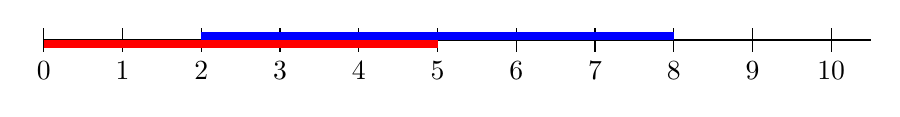
\begin{tikzpicture}%[x=1.2cm,y=1cm]

    % As
    \draw[thick] (0,0) -- (10.5,0);

    % Ticks
    \foreach \x in {0,1,2,3,4,5,6,7,8,9,10} {
        \draw (\x,-0.15) -- (\x,0.15);
        \node[below] at (\x,-0.15) {\x};
    }

    % Rood: tot 4
    \draw[line width=3pt, red] (0,-.05) -- (5,-.05);
    \draw[line width=3pt, red] (0,-.05) -- (5,-.05);

    % Blauw: vanaf 3 tot 5
    \draw[line width=3pt, blue] (2,.05) -- (8,0.05);

\end{tikzpicture}
\begin{tikzpicture}
\usetikzlibrary {datavisualization.formats.functions}
\def\mytypesetter#1{%
  \pgfmathparse{#1/pi}%
  \pgfmathprintnumber{\pgfmathresult}$\pi$%
}
\tikz \datavisualization
  [school book axes, all axes={unit length=1.25cm},
   x axis={ticks={step=(0.5*pi), tick typesetter/.code=\mytypesetter{##1}}},
   y axis={include value={-1,1}},
   visualize as smooth line]
  data [format=function] {
    var x : interval [0.5:7];
    func y = sin(\value x r);
  };
\end{tikzpicture}
\end{document}
